% SPDX-License-Identifier: CC BY 4.0
% Copyright (c) 2026 Fredrik Bierich
\documentclass[a4paper,12pt]{report}
\usepackage{amsmath}
\usepackage{amssymb}
\usepackage[margin=1in]{geometry}
\usepackage{graphicx}
\usepackage{lmodern}
\usepackage{pdflscape}
\usepackage{subcaption}
\usepackage{tikz}
\usepackage{titlesec}
\usepackage[hidelinks, colorlinks=true, urlcolor=blue, implicit=false]{hyperref}
\usepackage{hyperxmp}
\usepackage{orcidlink}
\hypersetup{
    pdfauthor={Fredrik Bierich},
    pdftitle={The Abstraction Gap Between Mathematics and Physics: A Geometric Perspective on Dimensional Analysis - A Summary},
    pdfsubject={Mathematics, Mathematical Physics},
    pdfkeywords={Dimensional Analysis, Circular Sector, Circular Functions, Arcus Functions, Chebyshev Polynomials, Simple Harmonic Motion, Uniform Circular Motion},
    pdfcopyright={Copyright © 2026 Fredrik Bierich},
    pdflicenseurl={https://creativecommons.org}
}
\graphicspath{{./output/}}
\setcounter{secnumdepth}{4}
\titleformat{\paragraph}[hang]{\normalfont\normalsize\bfseries}{\theparagraph}{1em}{}
\DeclareMathOperator{\arc}{arc}
\DeclareMathOperator{\area}{area}
\newcommand{\email}[1]{%
    {%
        \hypersetup{urlcolor=black}%
        \href{mailto:#1}{\nolinkurl{#1}}%
    }%
}
\title{The Abstraction Gap Between Mathematics and Physics: A Geometric Perspective on Dimensional Analysis - A Summary}
\author{Fredrik Bierich \orcidlink{https://orcid.org/0009-0008-0263-0950} \\ \email{fredrik.bierich@gmail.com}}
\date{\today \\ Copyright © 2026 Fredrik Bierich \\ Licensed under \href{https://creativecommons.org}{CC BY 4.0}}
\begin{document}
\maketitle
\section{Circular Sector}
\subsection{Arc Length}
\begin{subequations}
\begin{gather}
s = \lim \limits_{n \to \infty} 2^n \sqrt{2r^2 - 2ra_n} \\
a_n = \frac{\sqrt{2r^2 + 2ra_{n-1}}}{2}, n \geq 1 \\
a_0 = x, -r \leq x \leq r
\end{gather}
\end{subequations}
\subsection{Circular \& Arcus Functions}
\begin{equation}
\begin{aligned}
\cos \colon \mathbb{R}^{+} \times \mathbb{R} & \to \mathbb{R} \\
(r,s) & \mapsto x \in [-r,r]
\end{aligned}
\end{equation}
\begin{equation}
\cos(r,s) = r \sum \limits_{k=0}^{\infty} \frac{(-1)^k \left(\frac{s}{r}\right)^{2k}}{(2k)!}
\end{equation}
\begin{equation}
Q_r \stackrel{\text{def}}{=} \min \left\{s \in \mathbb{R}^+ \mid \cos(r,s) = 0\right\}
\end{equation}
\begin{equation}
\begin{aligned}
\sin \colon \mathbb{R}^{+} \times \mathbb{R} & \to \mathbb{R} \\
(r,s) & \mapsto y \in [-r,r]
\end{aligned}
\end{equation}
\begin{equation}
\sin(r,s) = r \sum \limits_{k=0}^{\infty} \frac{(-1)^k \left(\frac{s}{r}\right)^{2k+1}}{(2k+1)!}
\end{equation}
\begin{equation}
\begin{aligned}
\arccos \colon \{(r,x) \in \mathbb{R}^{+} \times \mathbb{R} \mid -r \leq x \leq r\} & \to \mathbb{R} \\
(r,x) & \mapsto s \in \left[0, 2Q_r\right]
\end{aligned}
\end{equation}
\begin{subequations}
\begin{gather}
\arccos(r,x) = \lim \limits_{n \to \infty} 2^n \sqrt{2r^2 - 2ra_n} \\
a_n = \frac{\sqrt{2r^2 + 2ra_{n-1}}}{2}, n \geq 1 \\
a_0 = x
\end{gather}
\end{subequations}
\begin{equation}
\begin{aligned}
\arcsin \colon \{(r,y) \in \mathbb{R}^{+} \times \mathbb{R} \mid -r \leq y \leq r\} & \to \mathbb{R} \\
(r,y) & \mapsto s \in \left[-Q_r, Q_r\right]
\end{aligned}
\end{equation}
\begin{equation}
\arcsin(r,y) = \frac{\arccos(r,-y) - \arccos(r,y)}{2}
\end{equation}
\subsection{Area}
\begin{equation}
A = \frac{rs}{2}
\end{equation}
\clearpage
\begin{figure}[p]
\centering
\resizebox{\textwidth}{!}{% Title: Figure 1
% Creator: GL2PS 1.4.2, (C) 1999-2020 C. Geuzaine
% For: Octave
% CreationDate: Wed Nov 25 13:38:39 2026
\setlength{\unitlength}{1pt}
\begin{picture}(0,0)
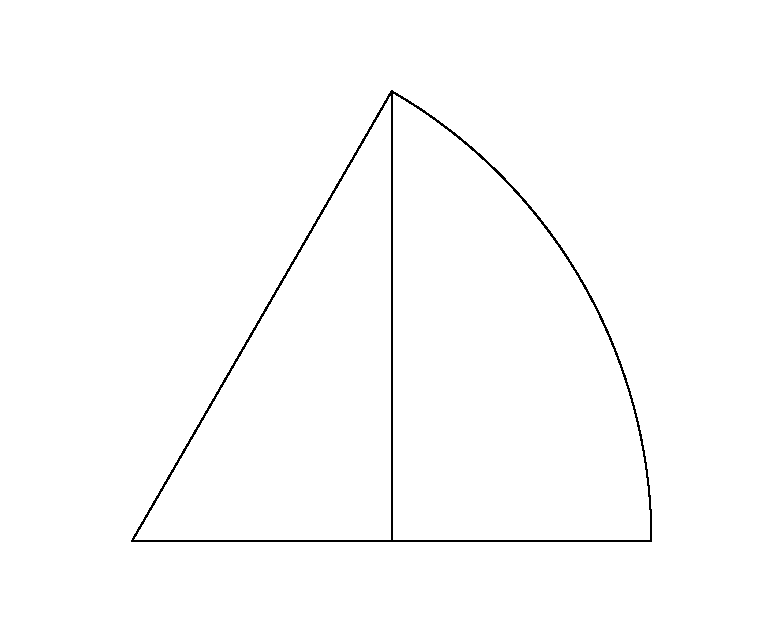
\includegraphics[scale=1]{circular_sector-inc}
\end{picture}%
\begin{picture}(360,288)(0,0)
\fontsize{12}{0}\selectfont\put(97.0695,158.213){\makebox(0,0)[l]{\textcolor[rgb]{0,0,0}{{$r$}}}}
\fontsize{12}{0}\selectfont\put(284.38,173.328){\makebox(0,0)[l]{\textcolor[rgb]{0,0,0}{{$s$}}}}
\fontsize{12}{0}\selectfont\put(113.905,14.1263){\makebox(0,0)[l]{\textcolor[rgb]{0,0,0}{{$x$}}}}
\fontsize{12}{0}\selectfont\put(199.33,143.498){\makebox(0,0)[l]{\textcolor[rgb]{0,0,0}{{$y$}}}}
\end{picture}
}
\caption{Circular sector.}
\end{figure}
\clearpage
\section{Simple Harmonic Motion}
\begin{equation}
[m] = \text{kg}
\end{equation}
\begin{equation}
[\omega] = \text{m/s}
\end{equation}
\begin{equation}
[k] = \text{N/m}
\end{equation}
\begin{equation}
[r] = \text{m}
\end{equation}
\begin{equation}
\omega = \left.\pm \left(\lim_{\Delta t \to 0} \frac{\Delta x}{\Delta t}\right)\right|_{x=0}
\end{equation}
\begin{equation}
T = \frac{4Q_r}{|\omega|}
\end{equation}
\begin{equation}
F = ma = -kx
\end{equation}
\begin{equation}
x(t) = \cos(r,\omega t)
\end{equation}
\begin{equation}
v(t) = \frac{dx}{dt} = \frac{-\omega \sin(r,\omega t)}{r}
\end{equation}
\begin{equation}
a(t) = \frac{dv}{dt} = \frac{-\omega^2 \cos(r,\omega t)}{r^2}
\end{equation}
\begin{equation}
m \omega^2 = kr^2
\end{equation}
\begin{equation}
K(t) = \frac{mv^2(t)}{2} = \frac{k \sin^2(r,\omega t)}{2}
\end{equation}
\begin{equation}
U(t) = \frac{kx^2(t)}{2} = \frac{k \cos^2(r,\omega t)}{2}
\end{equation}
\begin{equation}
E = K + U = \frac{m \omega^2}{2}
\end{equation}
\clearpage
\begin{figure}[p]
\centering
\resizebox{\textwidth}{!}{% Title: Figure 1
% Creator: GL2PS 1.4.2, (C) 1999-2020 C. Geuzaine
% For: Octave
% CreationDate: Sat Nov 28 10:08:10 2026
\setlength{\unitlength}{1pt}
\begin{picture}(0,0)
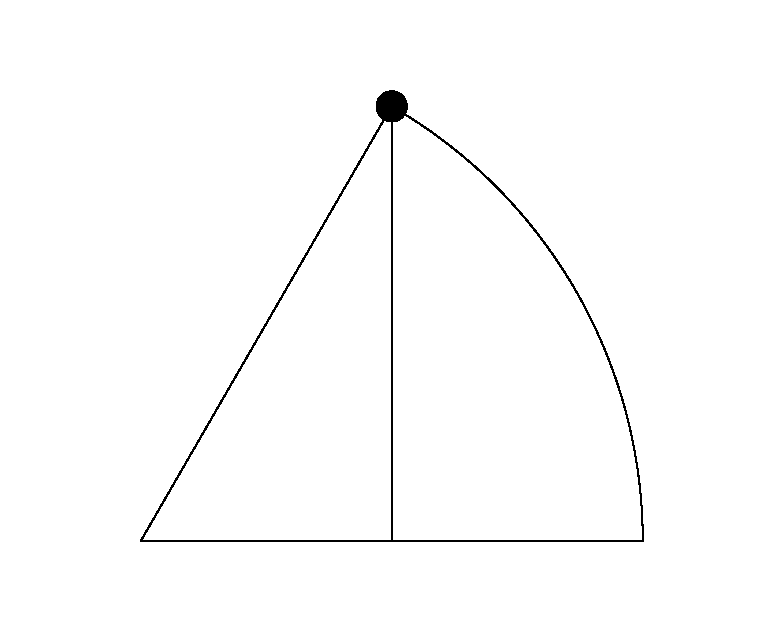
\includegraphics[scale=1]{uniform_circular_motion_spatial_position_diagram-inc}
\end{picture}%
\begin{picture}(360,288)(0,0)
\fontsize{12}{0}\selectfont\put(99.8458,154.122){\makebox(0,0)[l]{\textcolor[rgb]{0,0,0}{{$r$}}}}
\fontsize{12}{0}\selectfont\put(280.886,168.731){\makebox(0,0)[l]{\textcolor[rgb]{0,0,0}{{$s$}}}}
\fontsize{12}{0}\selectfont\put(116.118,14.8586){\makebox(0,0)[l]{\textcolor[rgb]{0,0,0}{{$x$}}}}
\fontsize{12}{0}\selectfont\put(198.683,139.899){\makebox(0,0)[l]{\textcolor[rgb]{0,0,0}{{$y$}}}}
\end{picture}
}
\caption{Uniform circular motion (spatial position diagram).}
\end{figure}
\clearpage
\begin{figure}[p]
\centering
\resizebox{\textwidth}{!}{% Title: Figure 1
% Creator: GL2PS 1.4.2, (C) 1999-2020 C. Geuzaine
% For: Octave
% CreationDate: Sat Nov 28 10:08:09 2026
\setlength{\unitlength}{1pt}
\begin{picture}(0,0)
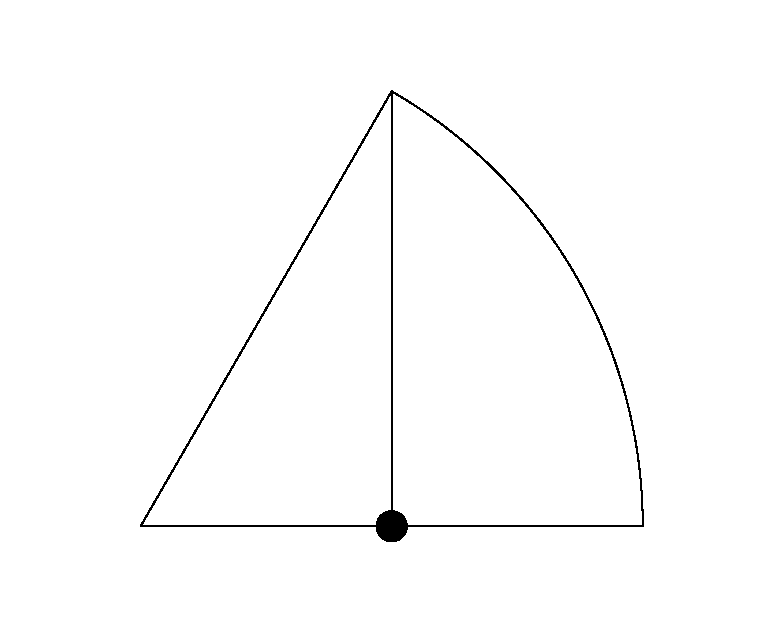
\includegraphics[scale=1]{simple_harmonic_motion-inc}
\end{picture}%
\begin{picture}(360,288)(0,0)
\fontsize{10}{0}\selectfont\put(36,28.5){\makebox(0,0)[t]{\textcolor[rgb]{0.15,0.15,0.15}{{$-\frac{3T}{4}$}}}}
\fontsize{10}{0}\selectfont\put(180,28.5){\makebox(0,0)[t]{\textcolor[rgb]{0.15,0.15,0.15}{{$-\frac{T}{4}$}}}}
\fontsize{10}{0}\selectfont\put(324,28.5){\makebox(0,0)[t]{\textcolor[rgb]{0.15,0.15,0.15}{{$\frac{T}{4}$}}}}
\fontsize{10}{0}\selectfont\put(31,36){\makebox(0,0)[r]{\textcolor[rgb]{0.15,0.15,0.15}{{$-r$}}}}
\fontsize{10}{0}\selectfont\put(31,144){\makebox(0,0)[r]{\textcolor[rgb]{0.15,0.15,0.15}{{$0$}}}}
\fontsize{10}{0}\selectfont\put(31,252){\makebox(0,0)[r]{\textcolor[rgb]{0.15,0.15,0.15}{{$r$}}}}
\fontsize{12}{0}\selectfont\put(180,12.5){\makebox(0,0)[t]{\textcolor[rgb]{0.15,0.15,0.15}{{$t$}}}}
\fontsize{12}{0}\selectfont\put(8.00001,144){\rotatebox{90}{\makebox(0,0)[b]{\textcolor[rgb]{0.15,0.15,0.15}{{$x(t) = \cos(r,\omega t)$}}}}}
\fontsize{10}{0}\selectfont\put(72.0912,200.7){\makebox(0,0)[l]{\textcolor[rgb]{0,0,0}{{$\omega = \lim \limits_{\Delta t \to 0} \frac{\Delta x}{\Delta t}$}}}}
\end{picture}
}
\caption{Simple harmonic motion.}
\end{figure}
\clearpage
\section{Uniform Circular Motion}
\begin{equation}
[m] = \text{kg}
\end{equation}
\begin{equation}
[\omega] = \text{m/s}
\end{equation}
\begin{equation}
[r] = \text{m}
\end{equation}
\begin{equation}
\omega = \lim \limits_{\Delta t \to 0} \frac{\Delta s}{\Delta t}
\end{equation}
\begin{equation}
T = \frac{4Q_r}{|\omega|}
\end{equation}
\begin{equation}
x(t) = \cos(r,\omega t)
\end{equation}
\begin{equation}
y(t) = \sin(r,\omega t)
\end{equation}
\begin{equation}
\vec{r}(t) = (x,y) = (\cos(r,\omega t),\sin(r,\omega t))
\end{equation}
\begin{equation}
\vec{v}(t) = \frac{d \vec{r}}{dt} = \frac{\omega \left(-\sin(r,\omega t),\cos(r,\omega t)\right)}{r}
\end{equation}
\begin{equation}
\vec{a} = \frac{d^2 \vec{r}}{dt^2} = \frac{-\omega^2 \vec{r}}{r^2}
\end{equation}
\begin{equation}
\vec{F} = m \vec{a} = \frac{-m \omega^2 \vec{r}}{r^2}
\end{equation}
\begin{equation}
v = \left|\vec{v}\right| = \left|\omega\right|
\end{equation}
\begin{equation}
E = \frac{mv^2}{2} = \frac{m \omega^2}{2}
\end{equation}
\begin{equation}
a = \left|\vec{a}\right| = \frac{\omega^2}{r}
\end{equation}
\begin{equation}
F = ma = \frac{m \omega^2}{r}
\end{equation}
\clearpage
\begin{figure}[p]
\centering
\begin{subfigure}{\textwidth}
\centering
\resizebox{\textwidth}{!}{% Title: Figure 1
% Creator: GL2PS 1.4.2, (C) 1999-2020 C. Geuzaine
% For: Octave
% CreationDate: Sat Nov 28 10:08:10 2026
\setlength{\unitlength}{1pt}
\begin{picture}(0,0)
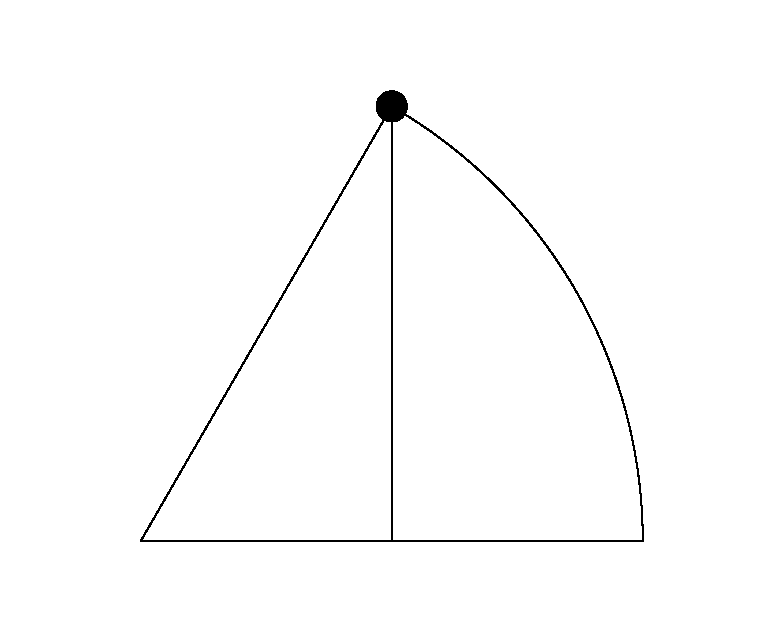
\includegraphics[scale=1]{uniform_circular_motion_spatial_position_diagram-inc}
\end{picture}%
\begin{picture}(360,288)(0,0)
\fontsize{12}{0}\selectfont\put(99.8458,154.122){\makebox(0,0)[l]{\textcolor[rgb]{0,0,0}{{$r$}}}}
\fontsize{12}{0}\selectfont\put(280.886,168.731){\makebox(0,0)[l]{\textcolor[rgb]{0,0,0}{{$s$}}}}
\fontsize{12}{0}\selectfont\put(116.118,14.8586){\makebox(0,0)[l]{\textcolor[rgb]{0,0,0}{{$x$}}}}
\fontsize{12}{0}\selectfont\put(198.683,139.899){\makebox(0,0)[l]{\textcolor[rgb]{0,0,0}{{$y$}}}}
\end{picture}
}
\caption{Spatial position diagram.}
\end{subfigure}
\caption{Uniform circular motion.}
\end{figure}
\clearpage
\begin{figure}[p]
\centering
\ContinuedFloat
\begin{subfigure}{\textwidth}
\centering
\resizebox{\textwidth}{!}{% Title: Figure 1
% Creator: GL2PS 1.4.2, (C) 1999-2020 C. Geuzaine
% For: Octave
% CreationDate: Fri Nov 20 13:34:27 2026
\setlength{\unitlength}{1pt}
\begin{picture}(0,0)
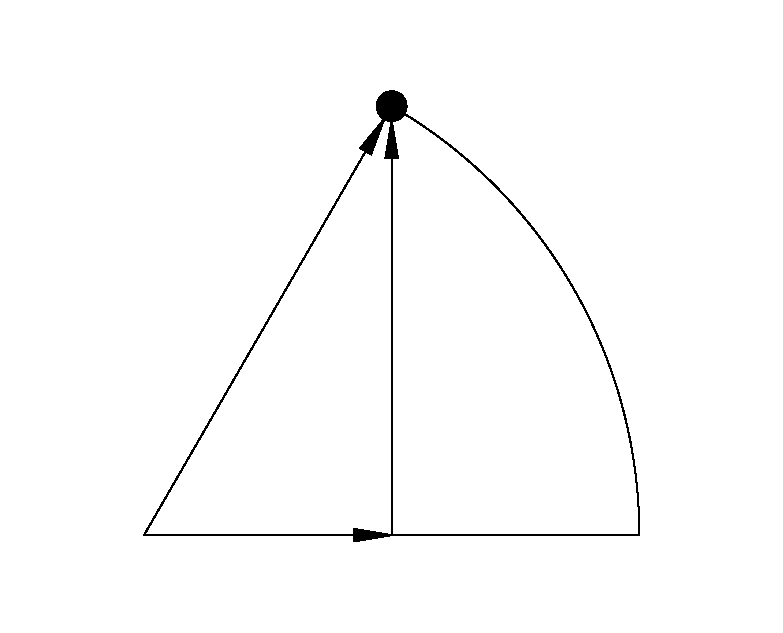
\includegraphics[scale=1]{uniform_circular_motion_position_vector_diagram-inc}
\end{picture}%
\begin{picture}(360,288)(0,0)
\fontsize{12}{0}\selectfont\put(100.949,155.469){\makebox(0,0)[l]{\textcolor[rgb]{0,0,0}{{$\vec{r}$}}}}
\fontsize{12}{0}\selectfont\put(279.498,169.876){\makebox(0,0)[l]{\textcolor[rgb]{0,0,0}{{$s$}}}}
\fontsize{12}{0}\selectfont\put(116.997,18.1213){\makebox(0,0)[l]{\textcolor[rgb]{0,0,0}{{$\vec{r}_x$}}}}
\fontsize{12}{0}\selectfont\put(198.426,141.441){\makebox(0,0)[l]{\textcolor[rgb]{0,0,0}{{$\vec{r}_y$}}}}
\end{picture}
}
\caption{Position vector diagram.}
\end{subfigure}
\caption{Uniform circular motion.}
\end{figure}
\end{document}
